\documentclass[aspectratio=169]{beamer}
\usetheme{TUDelft}

% ====================================================================
% ANIMATION TOGGLE
% ====================================================================
\newif\ifanimated
\animatedtrue
\ifdefined\staticmode
  \animatedfalse
\fi
\newcommand{\cpause}{\ifanimated\pause\fi}

% Packages
\usepackage{amsmath}
\usepackage{amssymb}
\usepackage{algorithm}
\usepackage{algorithmic}
\usepackage{graphicx}
\usepackage{tikz}
\usepackage{booktabs}
\usepackage{listings}
\usepackage{xcolor}
\usepackage{pifont}

% Python code styling
\lstset{
    language=Python,
    basicstyle=\ttfamily\footnotesize,
    keywordstyle=\color{blue},
    commentstyle=\color{gray},
    stringstyle=\color{red},
    showstringspaces=false,
    breaklines=true,
    frame=single,
    numbers=left,
    numberstyle=\tiny\color{gray}
}

% TikZ libraries
\usetikzlibrary{shapes,arrows,positioning,calc}

% Title information
\title[Embeddings \& Neural Ranking]{Embeddings and Neural Ranking}
\subtitle{Lecture 6: From Word2Vec to BERT}
\author{Avishek Anand}
\institute{Information Retrieval}
\date{\today}

\begin{document}

% Title slide
\begin{frame}
\titlepage
\end{frame}

% Course Context


% Outline
\begin{frame}{Outline}
\tableofcontents
\end{frame}

% ====================================================================
% SECTION 1: STATIC WORD EMBEDDINGS
% ====================================================================
\section{Word Embeddings (Static)}

\begin{frame}{Beyond One-Hot Encoding}
\begin{itemize}
    \item \textbf{Sparse:} One-hot vector ($[0, 0, 1, 0, \dots]$). $|V|$ dimensions. No similarity between "cat" and "dog".
    \item \textbf{Dense:} Low-dimensional vector ($v \in \mathbb{R}^{300}$). Capture semantics.
\end{itemize}

\vspace{1em}

\begin{block}{Distributional Hypothesis}
"You shall know a word by the company it keeps." (Firth, 1957)
\end{block}

\vspace{1em}
\begin{columns}
\begin{column}{0.48\textwidth}
\textbf{Word2Vec (Skip-gram):} \\
Predict context words given a target word.
\end{column}
\begin{column}{0.48\textwidth}
\textbf{GloVe:} \\
Global Vectors for Word Representation (matrix factorization + context).
\end{column}
\end{columns}
\end{frame}

\begin{frame}{Word2Vec: Skip-gram Intuition}
\begin{center}
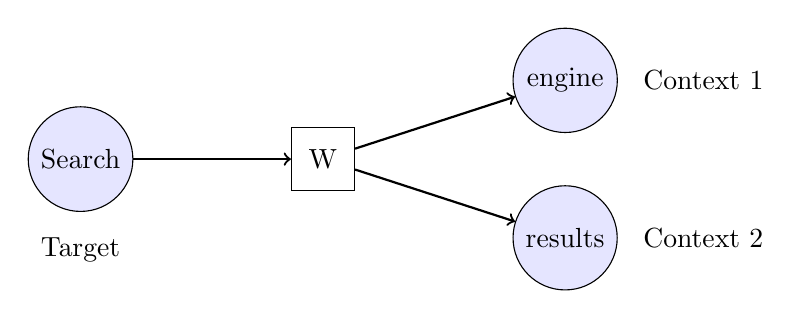
\begin{tikzpicture}[
    box/.style={rectangle, draw, minimum size=0.8cm},
    w/.style={circle, draw, fill=blue!10, minimum size=0.8cm},
    arrow/.style={->, thick}
]
    \node[w] (input) {Search};
    \node[box, right=2cm of input] (hidden) {$\text{W}$};
    \node[w, right=2cm of hidden, yshift=1cm] (out1) {engine};
    \node[w, right=2cm of hidden, yshift=-1cm] (out2) {results};
    
    \draw[arrow] (input) -- (hidden);
    \draw[arrow] (hidden) -- (out1);
    \draw[arrow] (hidden) -- (out2);
    
    \node[below=0.2cm of input] {Target};
    \node[right=0.2cm of out1] {Context 1};
    \node[right=0.2cm of out2] {Context 2};
\end{tikzpicture}
\end{center}

\vspace{1em}
\textbf{Limitation:} "bank" (river) and "bank" (finance) have the \textit{same} vector.
\end{frame}

% ====================================================================
% SECTION 2: CONTEXTUALIZED EMBEDDINGS \& TRANSFORMERS
% ====================================================================
\section{Contextualized Embeddings}

\begin{frame}{The Rise of Transformers}
\begin{itemize}
    \item \textbf{Self-Attention:} Every word in a sentence "looks" at every other word to build its representation.
    \item \textbf{Parallelization:} Unlike RNNs, Transformers process all words at once.
\end{itemize}

\vspace{1em}
\begin{center}
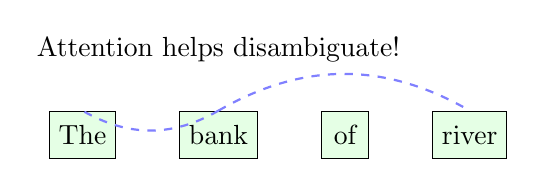
\begin{tikzpicture}[
    word/.style={rectangle, draw, fill=green!10, minimum size=0.6cm},
    att/.style={thick, blue!50, dashed}
]
    \node[word] (w1) {The};
    \node[word, right=0.8cm of w1] (w2) {bank};
    \node[word, right=0.8cm of w2] (w3) {of};
    \node[word, right=0.8cm of w3] (w4) {river};
    
    \draw[att] (w2.north) to[bend left] (w4.north);
    \draw[att] (w2.north) to[bend left] (w1.north);
    
    \node[above=0.5cm of w2] {Attention helps disambiguate!};
\end{tikzpicture}
\end{center}
\end{frame}

\begin{frame}{BERT: Bidirectional Encoder Representations}
\begin{block}{Pre-training: Masked Language Modeling (MLM)}
Hide 15\% of words and ask the model to predict them.
\texttt{"The [MASK] is cold today"} $\rightarrow$ \texttt{"weather"}
\end{block}

\vspace{1em}
\textbf{Why BERT for IR?}
\begin{itemize}
    \item Handles polysemy (different vectors for same word in different contexts).
    \item Deep understanding of syntax and nuances.
    \item \textbf{Cross-attention} between query and document.
\end{itemize}
\end{frame}

% ====================================================================
% SECTION 3: NEURAL RANKING ARCHITECTURES
) % ====================================================================
\section{Neural Ranking Architectures}

\begin{frame}{Bi-Encoders vs. Cross-Encoders}
\begin{columns}
\begin{column}{0.48\textwidth}
\begin{block}{Bi-Encoder}
\begin{itemize}
    \item Encode Q and D \textbf{independently}.
    \item Map to the same vector space.
    \item Score = Cosine Similarity / Dot Product.
    \item \textbf{Fast:} D can be pre-indexed.
\end{itemize}
\end{block}
\end{column}

\begin{column}{0.48\textwidth}
\begin{block}{Cross-Encoder}
\begin{itemize}
    \item Input: \texttt{[CLS] Q [SEP] D}
    \item Deep interaction (word-level) between Q and D.
    \item Score = BERT classifier output.
    \item \textbf{Slow:} Must process every pair at query time.
\end{itemize}
\end{block}
\end{column}
\end{columns}
\end{frame}

\begin{frame}{The Efficiency vs. Effectiveness Trade-off}
\begin{center}
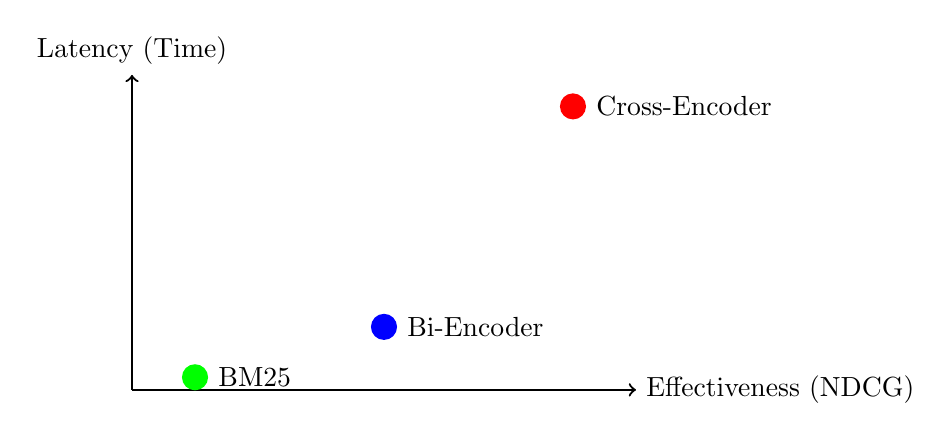
\begin{tikzpicture}[scale=0.8]
    \draw[->, thick] (0,0) -- (8,0) node[right] {Effectiveness (NDCG)};
    \draw[->, thick] (0,0) -- (0,5) node[above] {Latency (Time)};
    
    \node[circle, fill=red, label=right:Cross-Encoder] at (7, 4.5) {};
    \node[circle, fill=blue, label=right:Bi-Encoder] at (4, 1.0) {};
    \node[circle, fill=green, label=right:BM25] at (1, 0.2) {};
\end{tikzpicture}
\end{center}

\vspace{1em}
\textbf{Winner:} We usually use \textbf{both} in a multi-stage pipeline.
\end{frame}

% ====================================================================
% SECTION 4: MULTI-STAGE RE-RANKING
% ====================================================================
\section{Multi-Stage Re-ranking Flow}

\begin{frame}{The Standard IR Pipeline}
\begin{center}
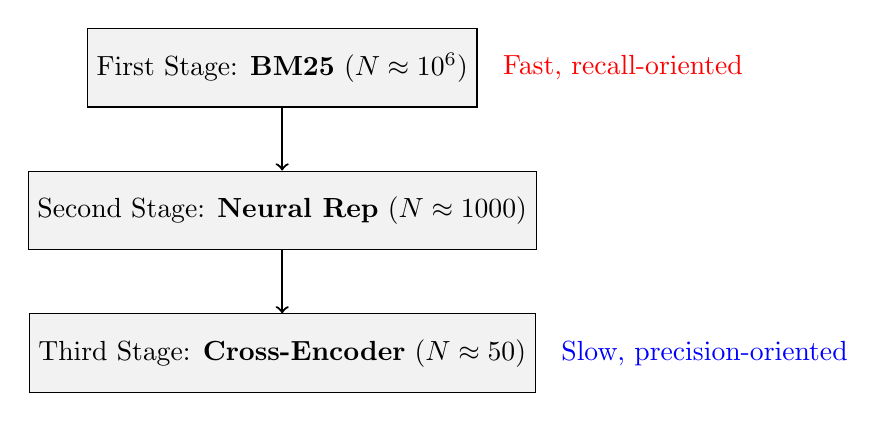
\begin{tikzpicture}[
    mystep/.style={rectangle, draw, fill=gray!10, minimum width=4cm, minimum height=1cm},
    arrow/.style={->, thick}
]
    \node[mystep] (s1) {First Stage: \textbf{BM25} ($N \approx 10^6$)};
    \node[mystep, below=0.8cm of s1] (s2) {Second Stage: \textbf{Neural Rep} ($N \approx 1000$)};
    \node[mystep, below=0.8cm of s2] (s3) {Third Stage: \textbf{Cross-Encoder} ($N \approx 50$)};
    
    \draw[arrow] (s1) -- (s2);
    \draw[arrow] (s2) -- (s3);
    
    \node[right=0.2cm of s1, text=red] {Fast, recall-oriented};
    \node[right=0.2cm of s3, text=blue] {Slow, precision-oriented};
\end{tikzpicture}
\end{center}
\end{frame}

\begin{frame}[fragile]{Neural Re-ranking in PyTerrier}
\begin{lstlisting}[language=Python]
import pyterrier as pt
# 1. BM25 Baseline
bm25 = pt.BatchRetrieve(index, wmodel="BM25")

# 2. Neural Re-ranker (e.g., MonoBERT)
# Takes top-100 from BM25 and re-ranks
monobert = pt.text.transformer.MonoBERT()
pipeline = bm25 % 100 >> monobert

# Run search
pipeline.search("what is neural ranking?")
\end{lstlisting}
\end{frame}

% ====================================================================
% SUMMARY
% ====================================================================
\section{Summary}

\begin{frame}{Key Takeaways}
\begin{itemize}
    \item[\checkmark] \textbf{Static Embeddings:} Capture semantics but miss context (polysemy).
    \item[\checkmark] \textbf{Transformers/BERT:} Context-aware representations via self-attention.
    \item[\checkmark] \textbf{Cross-Encoders:} Highly accurate but computationally expensive (word-word interaction).
    \item[\checkmark] \textbf{Bi-Encoders:} Fast, allow for pre-indexing (vector similarity).
    \item[\checkmark] \textbf{Re-ranking Pipeline:} Use fast methods (BM25) for recall, followed by neural methods for precision.
\end{itemize}

\vspace{1em}
\begin{center}
\textit{Next Lecture: Dense Retrieval \& Vector Similarity Search}
\end{center}
\end{frame}

\end{document}
